\documentclass[aspectratio=169,11pt]{beamer}

\usetheme{Singapore}
\usepackage[utf8]{inputenc}
\usepackage{amsmath}
\usepackage{amsfonts}
\usepackage{amssymb}
\usepackage{graphicx}
\usepackage{hyperref}
\usepackage{booktabs}

% Setup the bibliography
\usepackage[style=authortitle,backend=bibtex]{biblatex}
\addbibresource{bibliography.bib}
\setbeamertemplate{bibliography item}[text]
\setbeamerfont{footnote}{size=\tiny}

% Allow footnotes with no number
\newcommand\blfootnote[1]{%
  \begingroup
  \renewcommand\thefootnote{}\footnote{#1}%
  \addtocounter{footnote}{-1}%
  \endgroup
}

% Allow section title slides
\AtBeginSection[]{
  \begin{frame}
  \vfill
  \centering
  \begin{beamercolorbox}[sep=8pt,center,shadow=true,rounded=true]{title}
    \usebeamerfont{title}\insertsectionhead\par%
  \end{beamercolorbox}
  \vfill
  \end{frame}
}

\author{Dr Stephen Pederson}
\title{Lecture 4: Statistics For Transcriptomics}
\subtitle{BIOINF3005/7160: Transcriptomics Applications}
%\setbeamercovered{transparent} 
\setbeamertemplate{navigation symbols}{} 
\logo{
	
\includegraphics[scale=0.3]{figures/UoA_logo_col_vert.png} 
} 
\institute{Bioinformatics Hub, \\The University of Adelaide} 
\date{March 30th, 2020} 
\subject{BIOINF3005/7160: Transcriptomics Applications} 


\begin{document}

\begin{frame}
\titlepage
\end{frame}

\begin{frame}
\footnotesize
\tableofcontents
\end{frame}

\section{Introduction}

\begin{frame}{Introduction}

Today we'll 

	\begin{itemize}
		\item Discuss the relationship between our experiment and ``truth"
		\item Revise Hypothesis Testing
		\item Introduce strategies for managing error rates
		\item Introduce the moderated $T$-test
	\end{itemize}

\end{frame}	


\section{Sampling and the Null Hypothesis}


\begin{frame}{Sampling}

	Most experiments involve measuring something:\\[5mm]

	\begin{itemize}
		\item Continuous values e.g. Ct values, \textbf{fluorescence intensity}
		\begin{itemize}
			\item These values are often \textit{Normally distributed}
		\end{itemize}
		~\\[2mm]
	\pause
		\item Discrete values e.g. \textbf{read counts}, number of colonies
		\begin{itemize}
			\item These values often involve rates, i.e. colonies/$cm^2$
		\end{itemize}

	\end{itemize}

\end{frame}

\begin{frame}{Sampling}

	\begin{itemize}
		\item We are always interested in the \textbf{true underlying values} from the \textbf{entire population}
		\item We use our \textbf{sample-derived estimates} (i.e. from our data) to make inference about the \textbf{true values}
	\end{itemize}
		


\end{frame}

%\begin{frame}{Sampling}
%
%	Many data collections can also be considered as experimental datasets
%	
%	\begin{block}{Example 1}
%	In the 1000 Genomes Project a risk allele for T1D has a frequency of $\pi = 0.07$ in European Populations.
%	\end{block}
%	
%	~\\
%	\textbf{Does this mean, the allele occurs in exactly 7\% of Europeans?}
%
%\end{frame}
%
%\begin{frame}{Sampling}
%
%	\begin{block}{Example 2}
%	In our in vitro experiment, we found that 90\% of HeLa cells were lysed by exposure to our drug.
%	\end{block}
%	
%		\begin{itemize}
%			\item Does this mean that exactly 90\% of HeLa cells will always be destroyed?
%			\item What does this say about in vivo responses to the drug?
%		\end{itemize}
%
%\end{frame}

\begin{frame}{Population Parameters}

	\begin{itemize}
		\item Experimentally-obtained values represent an \textbf{estimate} of the true effect
		\begin{itemize}
			\item More formally referred to as \textit{population-level parameters}
		\end{itemize}
		\item Every experiment is considered a \textit{random sample of the complete population}
		\item Repeated experiments would give a \textbf{different} \textit{(but similar)} estimate
	\end{itemize}

\end{frame}

\begin{frame}{Hypothesis Testing}

In biological research we often ask:

	\begin{center}
	\textbf{“Is something happening?” or “Is nothing happening?”}
	\end{center}
	
	\pause

We might be comparing:

	\begin{itemize}
		\item Cell proliferation in response to antibiotics in media
		\item Methylation levels across genomic regions
		\item Allele frequencies in two populations
		\item \textbf{mRNA abundance in two related cell types}
	\end{itemize}

\end{frame}

\begin{frame}{Hypothesis Testing}

In biological research we often ask:

	\begin{center}
	\textbf{“Is something happening?” or “Is nothing happening?”}
	\end{center}

	How do we decide if our experimental results are “significant”?

	\begin{itemize}
		\item Do our measurements represent normal variability?
		\item What would the data look like if our \textit{experiment had no effect?}
		\item What would our data look like if there was \textit{some kind of effect?}
	\end{itemize}
	
	%\textbf{Every experiment is considered as a random sample from all possible repeated experiments.}

\end{frame}

\begin{frame}{The Null Hypothesis}

	\begin{itemize}
		\item The \textit{Null Hypothesis} ($H_0$) is used to describe the data if \textbf{nothing is happening}
		\item The \textit{Alternate Hypothesis} ($H_A$) captures \textbf{all other possibilities}
	\end{itemize}


\end{frame}

\begin{frame}{The Null Hypothesis}

	\begin{itemize}
		\item $H_0$: we have a test value (e.g. $\mu_0 = 0$) which allows us to define an expected distribution
		\begin{itemize}
			\item This test value represents our population statistic of interest (e.g. logFC)
		\end{itemize}
		\item $H_A$: Values which are unlikely to come from the defined $H_0$ distribution are assumed to come from $H_A$
		\begin{itemize}
			\item $H_A$ is every possibility besides no change $\implies$ \textit{we can't define this statistically}
		\end{itemize}
	\end{itemize}


\end{frame}

\section{The Sample Mean}

\begin{frame}{The Sample Mean}

For normally distributed data, we usually make inference about a \textbf{mean} of some type:

	\begin{itemize}
		\item We have an experiment-specific \textbf{estimate} of the \textit{mean logFC} ($\bar{x}$)
		\item We make inference about the \textbf{unknown} \textit{true mean logFC} ($\mu$)
		\item We use our `best guess' of the value we care about, e.g. $\mu_0 = 0$
		\pause
		\item In regression models, we fit \textbf{slope} and \textbf{intercept} terms 
		\begin{itemize}
			\item Principles introduced below are analogous: We \textit{estimate} a \textit{true} value
		\end{itemize}
	\end{itemize}


	\pause
	\begin{align*}
		\bar{x} \sim \mathcal{N}(\mu, \text{SE}_{\bar{x}})
	\end{align*}
	
	The \textit{standard error} of $\bar{x}$ (SE$_{\bar{x}}$) represents how variable this value is around $\mu$\\
	e.g. $SE_{\bar{x}} = \frac{\sigma}{\sqrt{n}}$, where $\sigma$ is population standard deviation


\end{frame}

\begin{frame}{The Sample Mean}

	\begin{itemize}
		\item If we know the population variance ($\sigma^2$), and have our sample size ($n$)
		\begin{itemize}
			\item We \textbf{almost never} know $\sigma$ and \textbf{never} know $\mu$
		\end{itemize}
		\item We can then use our \textit{value of interest}, e.g. $\mu_0 = 0$
		\begin{itemize}
			\item This is the value that we expect if $H_0$ is true
		\end{itemize}
	\end{itemize}

	\begin{align*}
	\bar{x} \sim \mathcal{N}(\mu_0, \frac{\sigma}{\sqrt{n}})
	\end{align*}


\end{frame}

\begin{frame}{The Sample Mean}

	\begin{align*}
		\bar{x} &\sim \mathcal{N}(\mu_0, \frac{\sigma}{\sqrt{n}})\\[3mm]
	\end{align*}

\end{frame}

\begin{frame}{The Sample Mean}

	\begin{align*}
		\bar{x} &\sim \mathcal{N}(\mu_0, \frac{\sigma}{\sqrt{n}})\\[3mm]
		\bar{x} - \mu_0 &\sim \mathcal{N}(0, \frac{\sigma}{\sqrt{n}}) \\[3mm]
	\end{align*}

\end{frame}

\begin{frame}{The Sample Mean}

	\begin{align*}
		\bar{x} &\sim \mathcal{N}(\mu_0, \frac{\sigma}{\sqrt{n}})\\[3mm]
		\bar{x} - \mu_0 &\sim \mathcal{N}(0, \frac{\sigma}{\sqrt{n}}) \\[3mm]
		Z = \frac{\bar{x} - \mu_0}{\frac{\sigma}{\sqrt{n}}} &\sim \mathcal{N}(0, 1)
	\end{align*}

\end{frame}

\section{Hypothesis Tests}

\begin{frame}{The Sample Mean}

If we know the population variance ($\sigma^2$), and have our sample size ($n$)

	\begin{align*}
		Z = \frac{\bar{x} - \mu_0}{\frac{\sigma}{\sqrt{n}}} \sim \mathcal{N}(0, 1)
	\end{align*}
	\begin{itemize}
		\item We use this as the underlying principle for $H_0$
		\item We don't know $\mu$ but we have a value ($\mu_0$) of interest (usually $\mu_0 = 0$)
	\end{itemize}
	~\\
	So if $H_0$ is true, \textbf{we know what kind of distribution our data will be drawn from}

\end{frame}

\begin{frame}{P Values}

	Once we can calculate a $Z$-score, we compare this to $\mathcal{N}(0, 1)$ and ask:\\
	
	\begin{center}
	\textbf{How likely are we to see this $Z$-score if $H_0$ is true?}	
	\end{center}

\end{frame}

\begin{frame}{P Values}

If we obtain $Z = 2$

	\begin{center}
		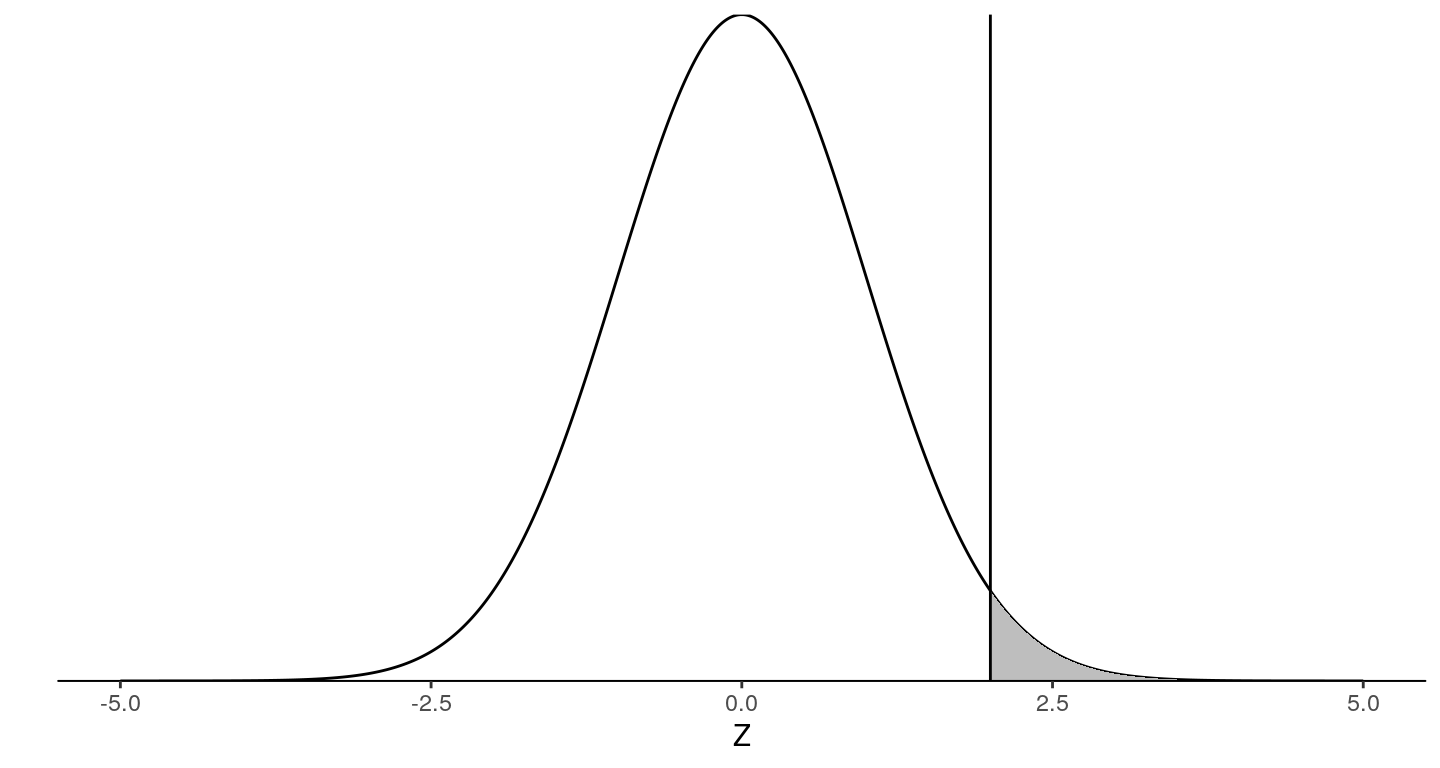
\includegraphics[scale=0.5]{figures/z2.png} 
	\end{center}

\end{frame}

\begin{frame}{P Values}
	\begin{itemize}
		\item The shaded area is the probability of obtaining $Z > 2$, assuming $H_0$ is true
		\item Most of the time we are look for $H_A: \mu_0 \neq 0$ so we need to look on \textit{both sides}
		\item This is known as a \textbf{two-sided test}
		\item Can also be described as $|Z| > 2$
	\end{itemize}
\end{frame}

\begin{frame}{P Values}

P$(|Z| > 2) = 0.0455$\\[5mm]

	\begin{center}
		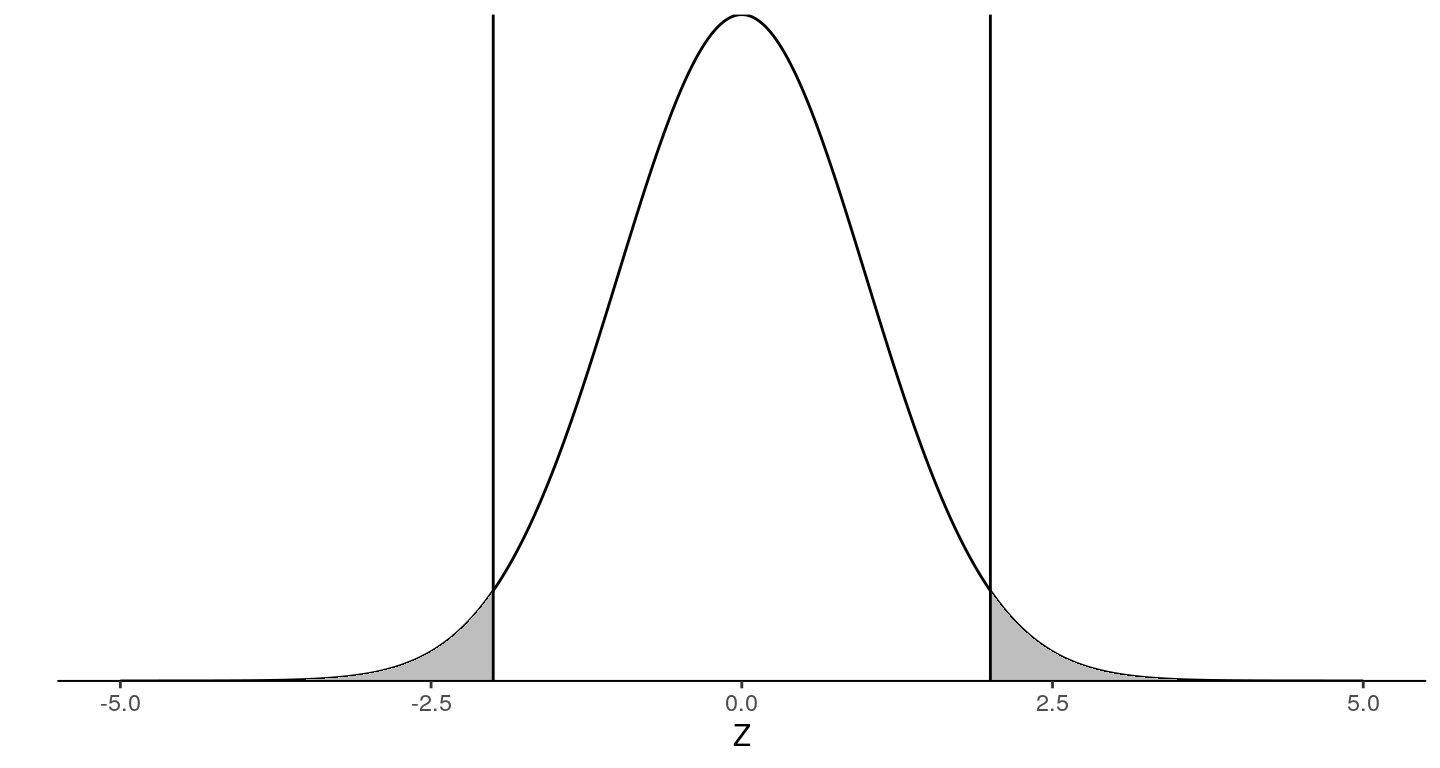
\includegraphics[scale=0.5]{figures/zAbs2.png} 
	\end{center}

\end{frame}

\begin{frame}{P Values}

P$(|Z| > 2) = 0.0455$\\[5mm]

	\begin{itemize}
		\item So if $H_0$ is true, we would see $Z > 2$ about 4.5 times every 100 experimental repeats
		\item We could then choose to accept $H_0$ as the most likely truth, or reject $H_0$ as the most likely truth
		\item How do we know if we have one of the 4.5 in 100?
		\pause
		\begin{itemize}
			\item We don't know
			\item Often set $p < 0.05$ as the rejection value (i.e. $\alpha = 0.05$)
		\end{itemize}
	\end{itemize}

\end{frame}

\begin{frame}{P Values}

	\begin{block}{Definition}
	A $p$-value is the probability of obtaining data as extreme, or more extreme than we have, if $H_0$ is true
	\end{block}

\end{frame}

\begin{frame}{Hypothesis Testing}

	\begin{enumerate}
		\item We have defined what our data should look like under $H_0$
		\item We have determined how likely we are to see our results
		\item We accept or reject $H_0$	if $p < \alpha$
	\end{enumerate}

\end{frame}

\begin{frame}{Hypothesis Testing}

In our context

	\begin{itemize}
		\item We are usually comparing $\mu_1$ against $\mu_2 \implies \mu_1 - \mu_2 = 0$
		\begin{itemize}
			\item This would be the expression level in two groups/conditions/treatments etc
			\item $\mu_1 - \mu_2 = 0$ is testing logFC $=0$
		\end{itemize}
		\pause
		\item We don't know the population variance ($\sigma$)
		\item We estimate $\sigma$ using our sample variance $\implies T$-tests
	\end{itemize}

\end{frame}

\begin{frame}{T-Tests}

A $T$-test is very similar to a $Z$-test

	\begin{align*}
		Z &= \frac{\bar{x} - \mu_0}{\frac{\sigma}{\sqrt{n}}} \sim \mathcal{N}(0, 1)\\
		T &= \frac{\bar{x} - \mu_0}{\frac{s}{\sqrt{n}}} \sim \mathcal{T}_{\nu}
	\end{align*}

The value $\nu$ means `degrees of freedom'

\end{frame}

\begin{frame}{The Sample Variance}

To calculate the sample variance ($s^2$) for a set of values $x = (x_1, x_2, \ldots, x_n)$

	\begin{align*}
		\bar{x} &= \frac{1}{n}\sum_{i = 1}^n x_i\\
		s^2 &= \frac{1}{n - 1}\sum_{i = 1}^n (x_i - \bar{x})^2
	\end{align*}

\end{frame}

\begin{frame}{Degrees of Freedom}

	\begin{itemize}
		\item The degrees of freedom ($\nu$) describe how `fat' the tails of a $T$-distribution are
		\begin{itemize}
			\item As $\nu \uparrow$ the tails become `less fat'\\[5mm]
		\end{itemize}
		\item The more individual samples we have ($n$), the more degrees of freedom we have
		\begin{itemize}
			\item The more samples we have, the less likely we are to see extreme values
			\item Commonly $\nu = n-1$
		\end{itemize}
	\end{itemize}

\end{frame}

\begin{frame}{T-Distributions}

	\begin{center}
		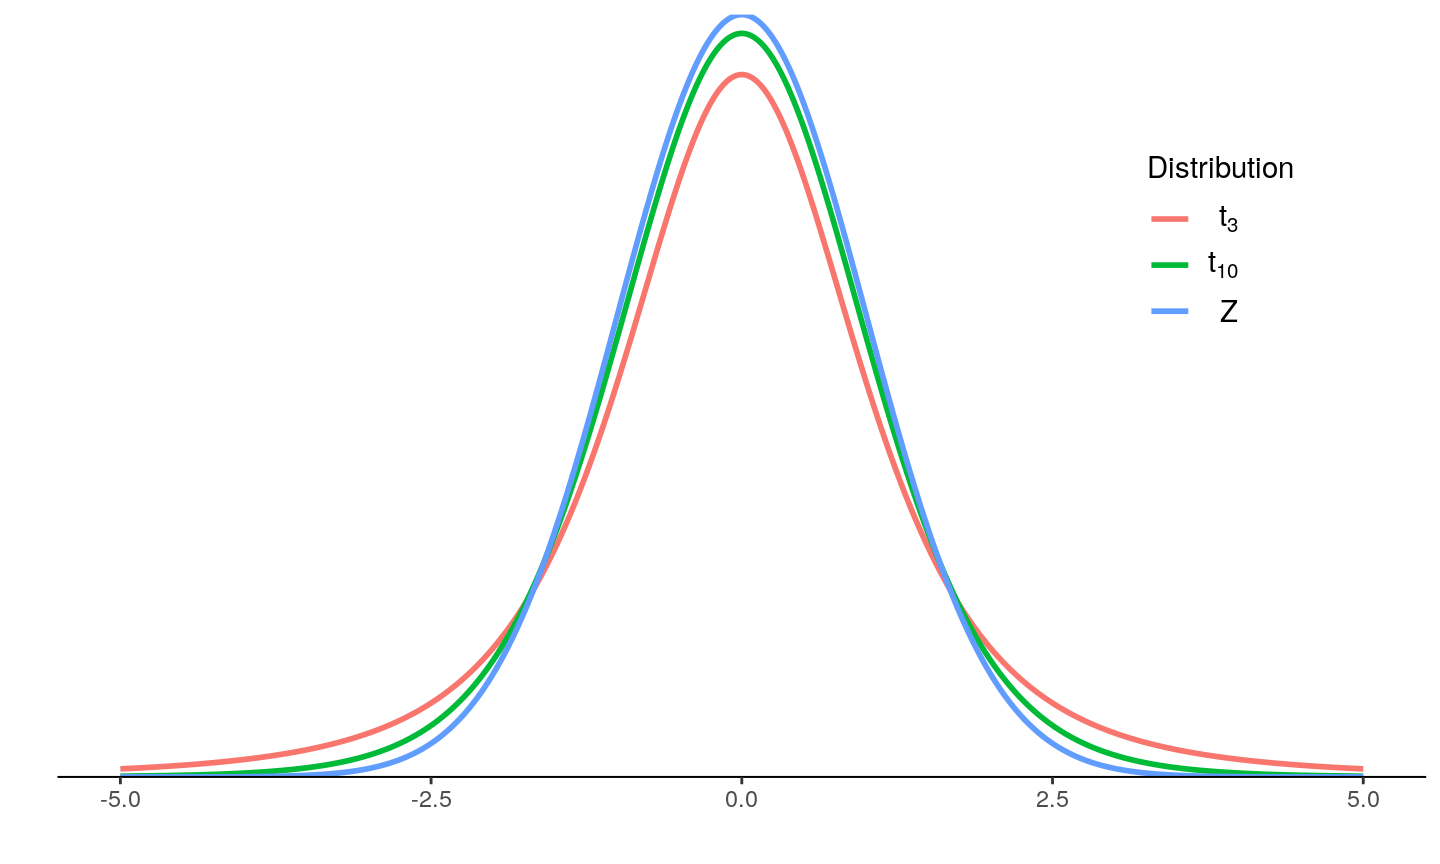
\includegraphics[scale=0.5]{figures/tvsz.png} 
	\end{center}

\end{frame}

\begin{frame}{T-Tests}

	\begin{enumerate}
		\item We now compare our $T$ statistic to the appropriate $T$ distribution
		\item Find the probability ($p$) of observing data as (or more) extreme if $H_0$ is true
		\item Accept or reject $H_0$	
	\end{enumerate}

\end{frame}

\begin{frame}{Transcriptomics}

	\begin{itemize}
		\item For Microarrays (i.e continuous data) we simply perform a $T$-test for every gene	
		\item Expression estimates are analysed on the $\log_2$ scale
	\end{itemize}
	
	\begin{align*}
	H_0: \mu_1 - \mu_2 = 0 \text{ Vs } H_A: \mu_1 \neq \mu_2
	\end{align*}
	
	\begin{itemize}
		\item The expression estimates $\bar{x_1}$ and $\bar{x_2}$ estimate $\mu_1$ and $\mu_2$
	\end{itemize}
	
\end{frame}

\begin{frame}{Transcriptomics}	
	
	\begin{itemize}
		\item We will also have a sample variance for each group $s_1$ and $s_2$
		\begin{itemize}
			\item Sample variances are assumed to be equal between groups
			\item We pool sample variances ($s_p = \ldots$)
			\item $\nu = n_1 + n_2 - 2$
		\end{itemize}
	\end{itemize}
	
	\begin{align*}
		T = \frac{\bar{x}_1 - \bar{x}_2}{s_p \sqrt{\frac{1}{n_1} + \frac{1}{n_2}}}
	\end{align*}
	
\end{frame}

\begin{frame}{Transcriptomics}

	\begin{itemize}
		\item We often have $k > 2$ groups $\implies$ multiple pairwise comparisons	
		\item Or some kind of regression model with discrete predictors (i.e. group-wise) 
	\end{itemize}
	
	\begin{align*}
		s_p^2 = \frac{\sum_{i=1}^k(n_i -1)s_i^2}{\sum_{i=1}^k(n_i -1)}
	\end{align*}
	
	In transcriptomics we usually refer to this as the \textit{residual variance}

\end{frame}

\section{Multiple Testing}

\begin{frame}{P Values}

	\begin{itemize}
		\item We perform `000's of $T$-tests in every experiment (one per gene)
		\item A $p$-value of 0.05 $\implies$ 1 in 20 times we will see data this (or more) extreme \textbf{if $H_0$ is true}
		\item A $p$-value of 0.01 $\implies$ 1 in 100 times we will see data this (or more) extreme \textbf{if $H_0$ is true}
		\item So if we have 10,000 genes \textbf{for which $H_0$ is true}, how many times will we see:
		\begin{itemize}
			\item $p < 0.05$
			\item $p < 0.01$
		\end{itemize}
	\end{itemize}

\end{frame}

\begin{frame}{P Values}

	\begin{itemize}
		\item We perform `000's of $T$-tests in every experiment (one per gene)
		\item A $p$-value of 0.05 $\implies$ 1 in 20 times we will see data this (or more) extreme \textbf{if $H_0$ is true}
		\item A $p$-value of 0.01 $\implies$ 1 in 100 times we will see data this (or more) extreme \textbf{if $H_0$ is true}
		\item So if we have 10,000 genes \textbf{for which $H_0$ is true}, how many times will we see:
		\begin{itemize}
			\item $p < 0.05 \implies \sim500$ times
			\item $p < 0.01 \implies \sim100$ times
		\end{itemize}
	\end{itemize}

\end{frame}

\begin{frame}{Error Rates}

	\begin{itemize}
		\item If we reject $H_0$ using $p < 0.05 \implies \sim500$ errors (false rejections)
		\item If we reject $H_0$ using $p < 0.01 \implies \sim100$ errors (false rejections)
	\end{itemize}
	
	~\\[3mm]
	These are known as \textit{Type I} errors
	
	\begin{itemize}
		\item In biological research, these can waste \$\$\$
		\item We need to control these errors
	\end{itemize}

\end{frame}

\begin{frame}{Error Rates}

	\begin{center}
		\begin{tabular}{r|l|l}
		\toprule
			& $H_0$ True & $H_0$ Not True \\
		\midrule
		Reject $H_0$ & Type I Error & \checkmark\\
		\midrule
		Accept $H_0$ & \checkmark & Type II Error \\
		\bottomrule
		\end{tabular}	
	\end{center}

~\\[3mm]
We need to \textbf{minimise both Type I and Type II} errors 

\end{frame}

\begin{frame}{Error Rates}

Two primary strategies for controlling error rates\\[5mm]

	\begin{enumerate}
		\item Bonferroni's Method
		\begin{itemize}
			\item This sets the bar very high to reject $H_0$
			\item Big increase in Type II errors
		\end{itemize}
		\item False Discovery Rate
		\begin{itemize}
			\item Allows a small number of false discoveries
			\item Reduces Type II errors (compared to Bonferroni)
		\end{itemize}
	\end{enumerate}


\end{frame}

\begin{frame}{Error Rate}

\textit{The Bonferroni Adjustment}

	\begin{itemize}
		\item If you have $m = 10,000$ tests and $\alpha = 0.05$
		\item Set $\alpha_{\text{bonf}} = \frac{\alpha}{m} = \frac{0.05}{10000} = 5\times10^{-7}$
		\item Alternatively, adjust each $p$-value: $p_{\text{bonf}} = \min(1, m*p)$\\[4mm]
	\end{itemize}

\pause
\textit{The Family-Wise Error Rate (FWER)}\\

	\begin{itemize}
		\item The effect is P(one Type I Error) $\leq 0.05$
		\item This is strict control of the \textit{family-wise error rate}
		\item The family is the complete set of $m$ tests
	\end{itemize}

\end{frame}

\begin{frame}{The False Discovery Rate}

	\begin{itemize}
		\item \textit{False Discovery Rate} strategies are very common in transcriptomics
		\item We allow a small amount of noise into our results $implies$ signal still swamps noise
		\begin{itemize}
			\item An $FDR = 0.05 \implies \leq 5$\% of our results are `false discoveries' (Type I Errors)
		\end{itemize}
		\item The most common method is the Benjamini-Hochberg method\footfullcite{BenjaminiHochbergFDR}
		\item Other methods include Storey's $q$-value\footfullcite{Storey9440}
		\item These methods \textbf{do not control} the \textit{FWER} but \textbf{do control} the \textit{FDR}
	\end{itemize}

\end{frame}

\section{Moderated $T$-tests}

\begin{frame}{Moderated $T$-tests}

	\begin{itemize}
		\item When conducting our $m$ simultaneous $T$-tests, we use an estimate of the population variance $s_p$\\[2mm]
		\begin{itemize}
			\item Some of these are going to be larger than the true population value
			\item Others are going to be smaller than the true population value	\\[4mm]
		\end{itemize}
		\pause
		\item What impact will this have?
	\end{itemize}

\end{frame}

\begin{frame}{Moderated $T$-tests}
	
	\begin{align*}
		T = \frac{\bar{x}_1 - \bar{x}_2}{s_p \sqrt{\frac{1}{n_1} + \frac{1}{n_2}}}
	\end{align*}
	
	\begin{itemize}
		\item If $s_p <<< \sigma \implies T\uparrow$ 
		\item We may get significant results with small logFC, due to small variances\\[2mm]
		\pause
		\item If $s_p >>> \sigma \implies T\downarrow$ 
		\item We will miss truly DE genes due to large variances
	\end{itemize}

\end{frame}

\begin{frame}{Moderated $T$-tests}

	\begin{itemize}
		\item This situation exists in \textbf{every} $T$-test
		\item In transcriptomics, we perform `000's in parallel
		\item We can take advantage of this $\implies$ \textit{Empirical Bayes} model
		\item This gives us a moderated value of $s_p$ $\implies$ \textit{Moderated $T$-test}\footfullcite{pmid16646809}
	\end{itemize}
	
\end{frame}

\begin{frame}{Moderated $T$-tests}	

		\begin{itemize}
			\item Variances are usually drawn from a Scaled Inverse $\chi^2$ distribution
			\item Given that we have `000's of genes, we can estimate the hyperparameters for a Bayesian Model
			\item We end up with a \textit{posterior estimate} known as the moderated variance ($\tilde{s}_p^2 = E[\sigma^2|s_p^2]$)
			\item Overestimates/Underestimates are shrunk towards the mean
			\item Increases Power ($\downarrow$ Type II Errors) and Decreases Type I Errors
		\end{itemize}

\end{frame}




%\section{Dimensional Reduction}


\end{document}
